\chapter{Implementering}
MANGLER TEKST!

\subsection{Brugergrænseflade}
Ved programmets opstart vises det statiske kort som gruppen har valgt at benytte under udviklingen af dette program, samt en load knap. Dette er at finde i tabben “Map View”. Tabben “Data View” vil ikke indeholde noget information ved opstart af programmet. Efter tryk på load knappen, popper en dialogbox op, hvorefter brugeren skal vælge den mappe som indeholder løbernes GPX-filer, samt koordinater for posterne til den bane løberne skal løbe. Dette kan ses på figur 7.1.

\begin{figure} [h]
	\centering
	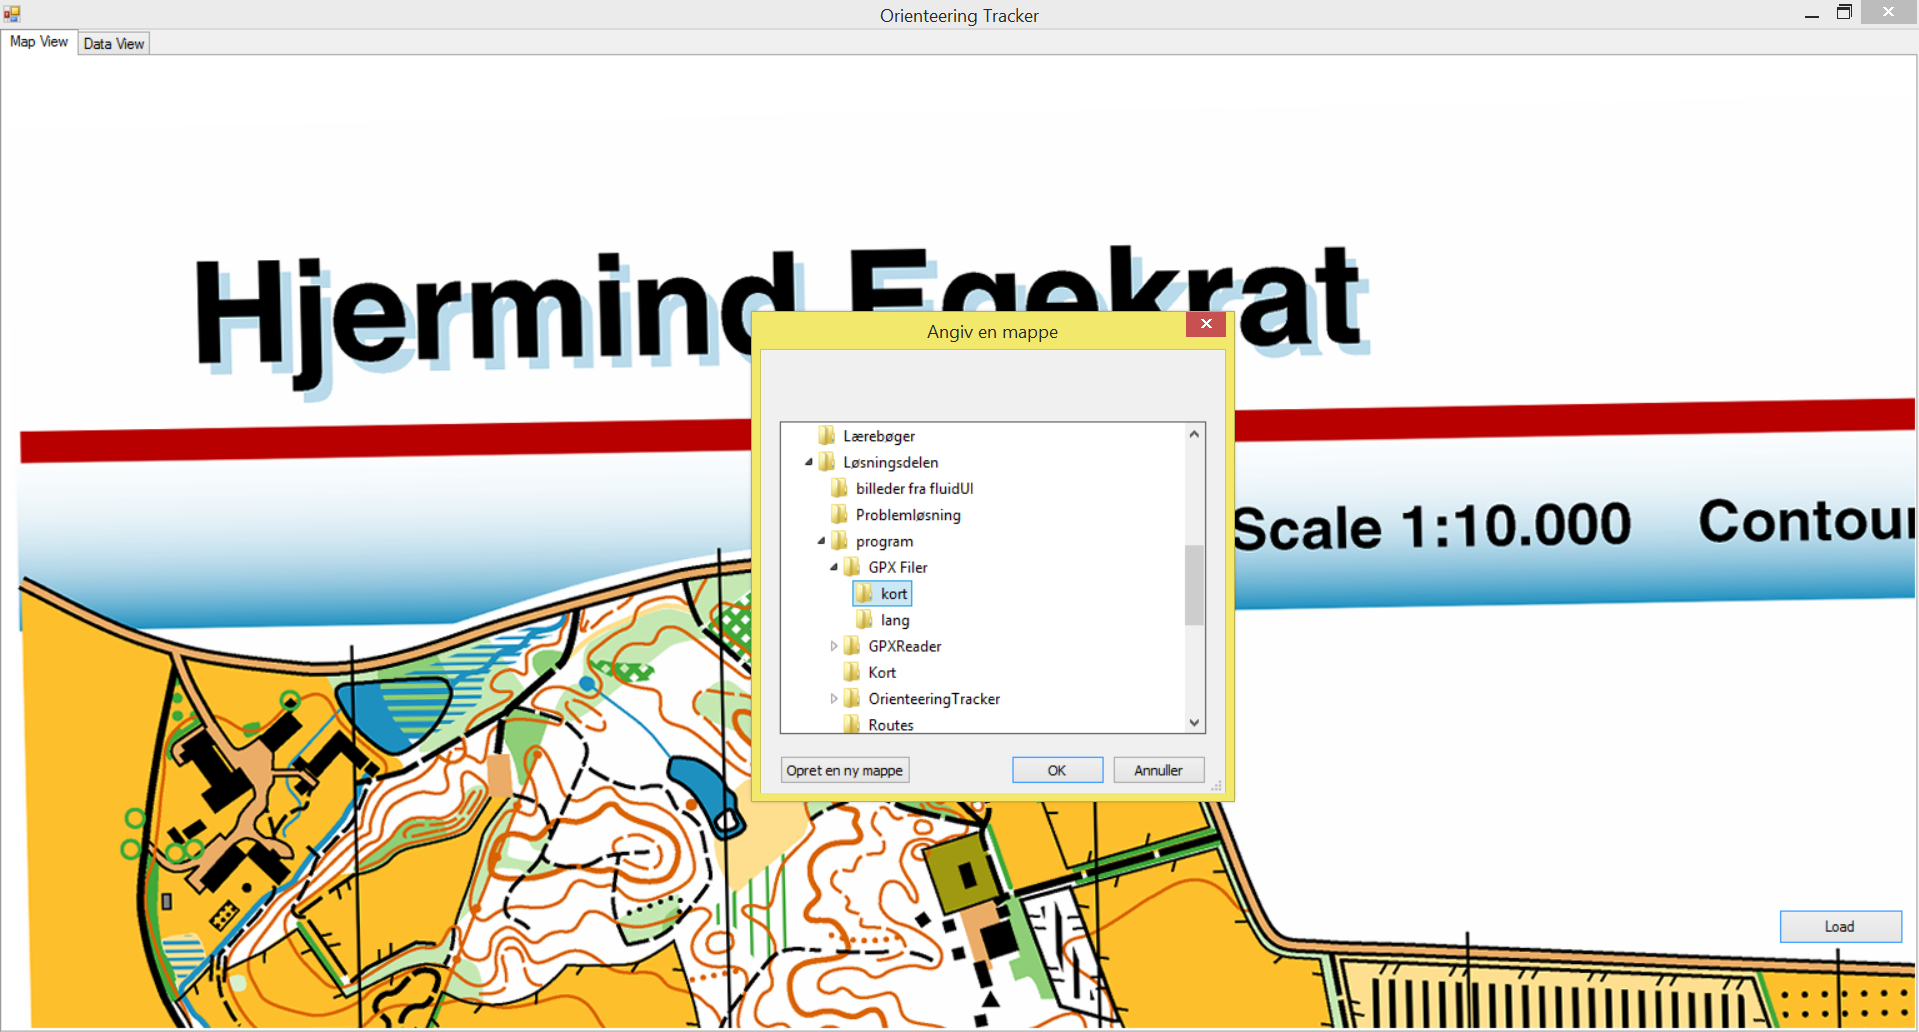
\includegraphics[width=1\textwidth]{billeder/MapView1}
	\caption{Klassediagram over projektets program}
\end{figure}

Når GPX-filer og koordinaterne for posterne er loadet ind i programmet, vil de forskellige mediaplayer funktioner komme frem, som ses på figur 7.2.

\begin{figure} [h]
	\centering
	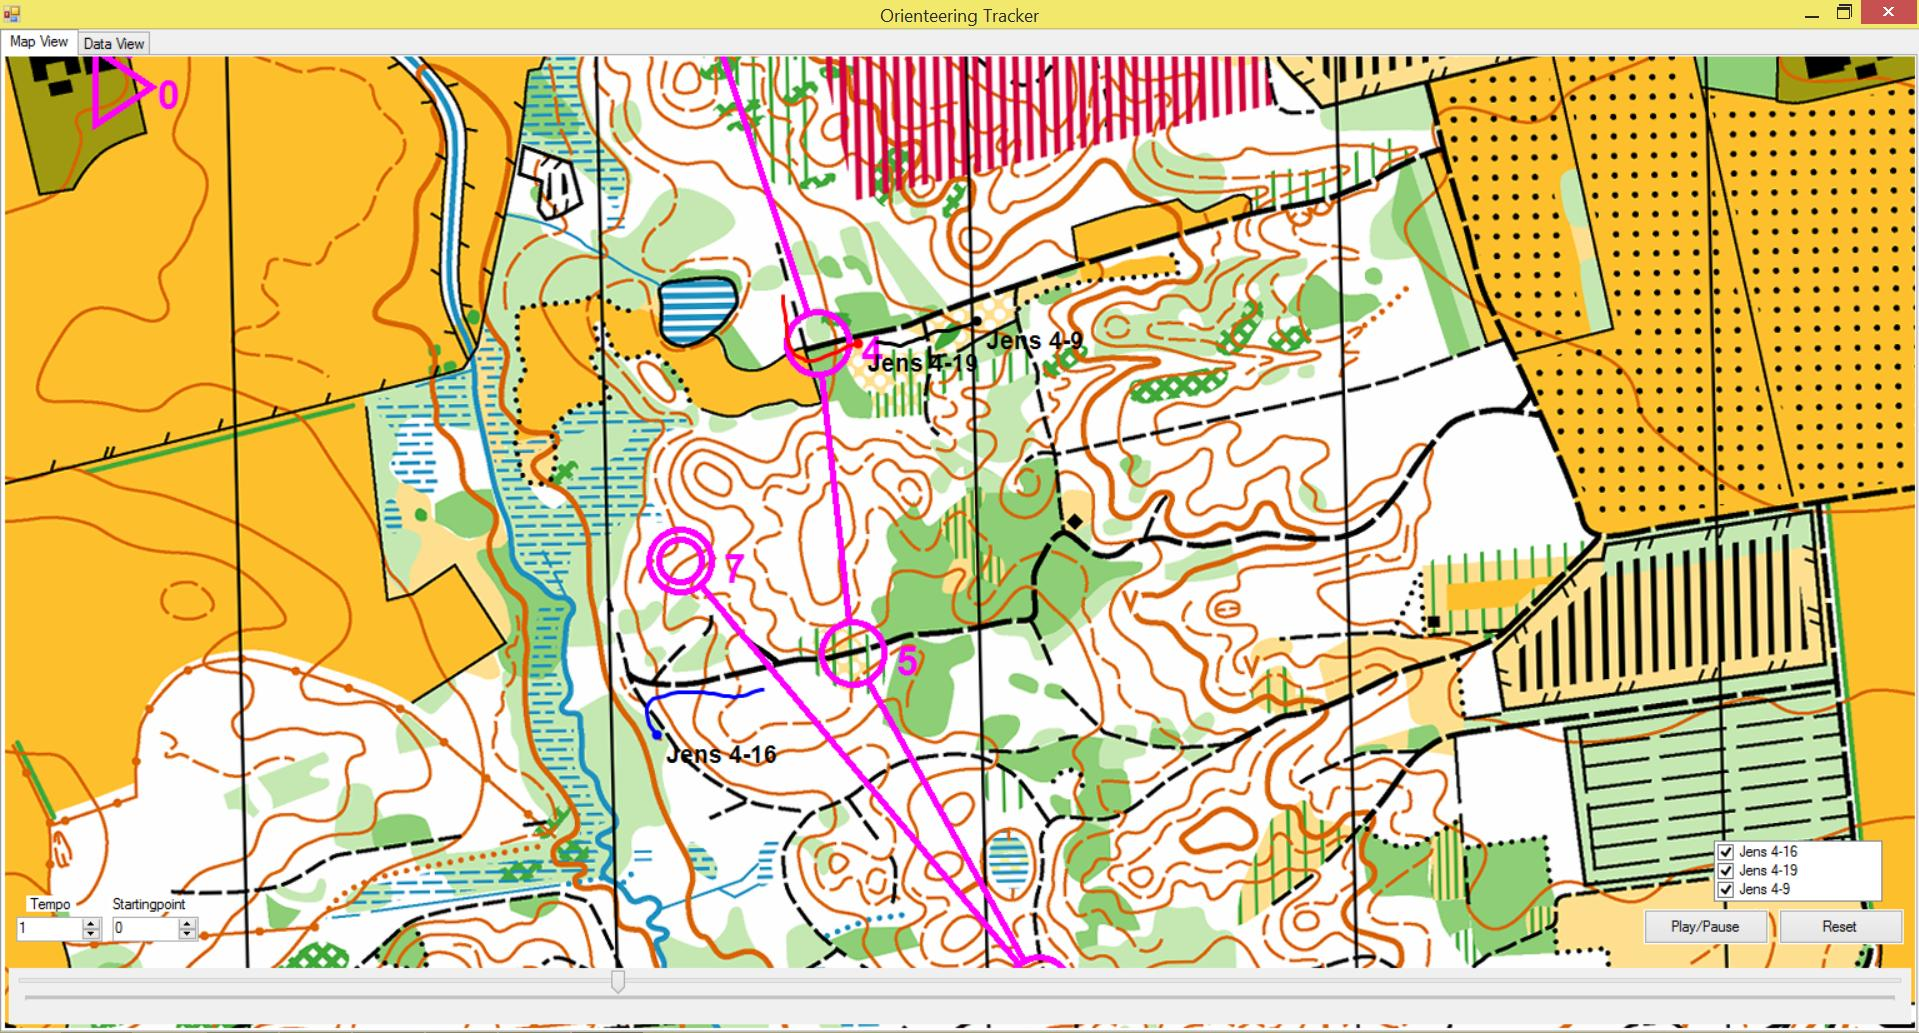
\includegraphics[width=1\textwidth]{billeder/MapView2}
	\caption{Klassediagram over projektets program}
\end{figure}

I bunden af programmet ses programmets trackbar, der gør det muligt at spole frem og tilbage under afspilningen. Nede i venstre hjørne findes to forskellige mediaplayer funktioner. Den yderste til venstre bruges til at vælge tempoet for afspilningen. Den anden bruges til at vælge startpost for løberne, hvilket gør det muligt at samle løberne, for lettere at kunne sammenligne dem med hinanden. På højre side ses en play/pause og  reset knap. Play/pause bruges til at starte/pause afspilningen. Reset knappen bringer programmet tilbage til dets opstarts stadie. Lige over disse to knapper findes en check box. I denne checkbox kan alle løberne ses. Checkboxen afgør hvilke løbere der vises på kortet, hvilket gør det muligt at skjule løbere, hvis der vil fokuseres på nogle bestemte løbere. Løberne vises ude på kortet med en prik i hver deres farve, samt en hale efter denne, som viser hvordan de har løbet de sidste 30 sekunder. 

Når der trykkes på tabben “Data View” vil alle løbernes data for løbet vises. I “Data View” kan der ses løbernes slut position, navn, tid, tidsdifference til førstepladsen, tilbagelagt distance, hastighed i minut pr. kilometer og tiden for hvert stræk. Der kan ses et eksempel på dette på figur 7.3 herunder. 
\begin{figure} [h]
	\centering
	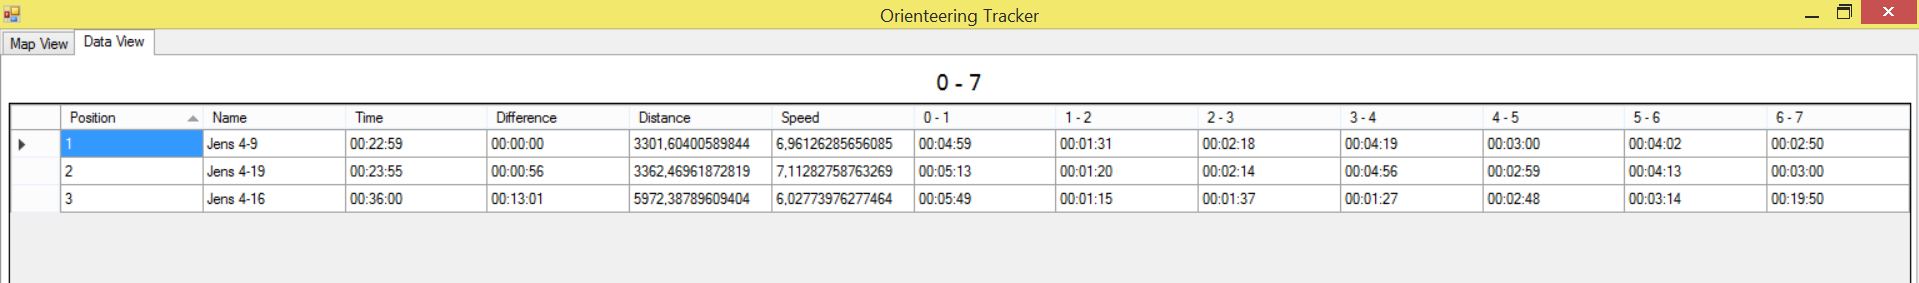
\includegraphics[width=1\textwidth]{billeder/DataView1}
	\caption{Klassediagram over projektets program}
\end{figure}

Klikkes der på et felt for et stræk, kan der ses mere detaljerede informationer om det specifikke stræk. Som det kan ses på figur 7.4, indeholder dette de samme informationer som når der ses på hele løbet, med en enkelt undtagelse, her kan løberne se hvilken position de fik på det specifikke stræk. 
\begin{figure} [h]
	\centering
	\includegraphics[width=1\textwidth]{billeder/DataView2}
	\caption{Klassediagram over projektets program}
\end{figure}

\section{Programstruktur}
Da ingen af medlemmerne i gruppen har tidligere erfaring med udvikling af store applikationer i C\# og Windows Forms, blev meget af udviklingen lavet ud fra “trial and error” princippet. Med det menes at gruppen forsøgte sig meget frem, for at lære at bruge Windows Forms, og der ikke blev lavet en decideret plan eller design for programmet, før udviklingen blev påbegyndt. Dette medførte at store dele af programmet blev lavet i samme klasse, hvilket forårsagede et forholdsvist lavt abstraktionsniveau. 

\subsection{Klassebeskrivelse}
Gruppen har vha. Visual Studio udarbejdet et klasse diagram, for at give et bedre overblik over programmets klasser. I firkanterne i klassediagrammet ses klassens navn, dens fields, properties og metoder.

\begin{figure} [h]
	\centering
	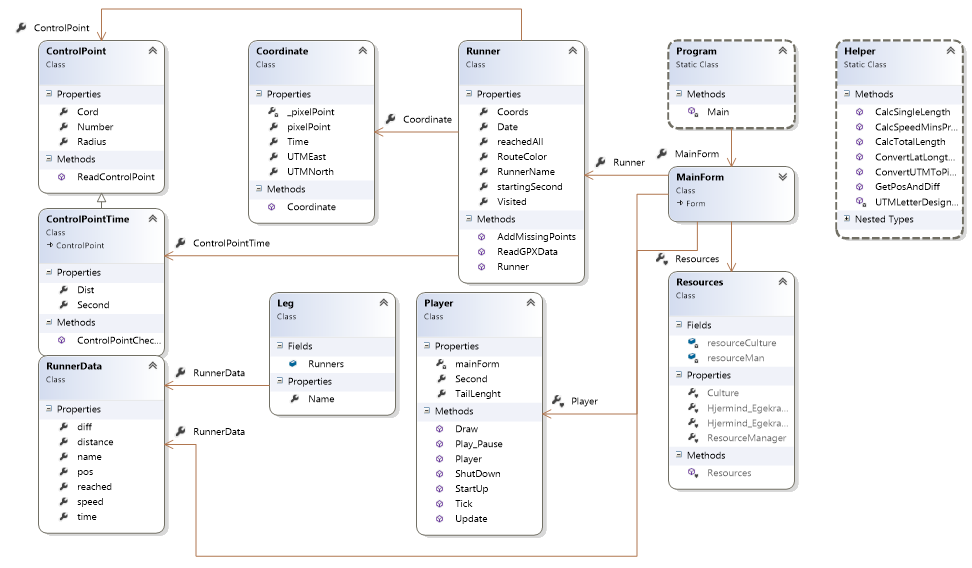
\includegraphics[width=1\textwidth]{billeder/KlasseDiagram}
	\caption{Klassediagram over projektets program}
\end{figure}

\begin {itemize}
\item \textbf{Helper} klassen indeholder de metoder der bruges til at lave udregninger i programmet, eksempelvis konverteringen fra længde- breddegrade koordinater til UTM koordinater. 
\item \textbf{Coordinate} indeholder koordinater for at kunne se hvor løberen er og hvor posterne er placeret, som både pixel- og UTM koordinater. 
\item \textbf{ControlPoint} repræsentere posterne i løbet. Hvor den indeholder en posts radius, dens nummer og henter dens koordinater fra Coordinates.
\item \textbf{ControlPointTime} har nedarvet fra ControlPoint, hvor den så implementere Second og Dist som vil være tid i sekunder og distancen fra løberen til posten. 
\item \textbf{Runner} indeholder informationer om en løber, dette er bl.a. løberens koordinater på ruten, om løberen har besøgt alle poster og løberens navn.
\item \textbf{RunnerData} gemmer på en mængde data om hver enkelt løber, som hastighed, distance løbet og position i løbet, hvor dette vil være de informationer som kan findes under tabben som gruppen har kaldt ”Data view”. 
\item \textbf{Leg} er det som førnævnt kaldet et ”stræk”, dog nu oversat til engelsk. Leg indeholder en list af RunnerData samt et navn på strækket.
\item \textbf{Player} sørger for at tegne løberen på kortet, samt den hale som skal være efter løberen. Derudover viser, skjuler og opdatere den forskellige funktioner i programmet når det køres, dette bruges i den tab som gruppen har kaldt ”Map view”.
\item \textbf{MainForm} holder sammen på programmet. Det er er GUI’en bliver lavet, samt events til programmet. 
\item \textbf{Resources} indeholder kortet som bruges I programmet, samt worldfilen.
\end {itemize}

MANGLER NOGET TEKST HER?

\section{Kildekoden}
TEKST HER!

\subsection{Helper}
Helper er en statisk klasse, der er lavet for at have nogle funktioner tilgængelige overalt i programmet, uden at skulle instantiere et nyt objekt der kunne udføre handlingerne, eller copy-paste funktionerne ind i de klasser der skal bruge dem. 

Helper indeholder konverteringsfunktionerne, i henholdsvis ConvertLatLongToUTM, og ConvertUTMToPixel. ConvertLatLongToUTM funktionen, er lånt fra brugeren Hactic fra Worldwindcentral's forum \citep{UTM}.
Derudover bliver Helper klassen også brugt til at lave beregninger på løbernes ture, altså distance og hastighedsberegninger.
 
ConvertUTMToPixel metoden konvertere UTM

\begin{lstlisting}
public static void ConvertUTMToPixel(double UTM_north, double UTM_east, out float x, out float y)
{
    MemoryStream ms = new MemoryStream(OrienteeringTracker.Properties.Resources.Hjermind_Egekrat_ref_ref1);
    string line;
    List<float> worldTal = new List<float>();
    StreamReader sr = new StreamReader(ms, Encoding.UTF8);

    while ((line = sr.ReadLine()) != null)
    {
        worldTal.Add(float.Parse(line, CultureInfo.InvariantCulture));
    }

    x = Convert.ToInt32((UTM_east - worldTal[4]) / worldTal[0]);
    y = Convert.ToInt32((UTM_north - worldTal[5]) / worldTal[3]);
}
\end{lstlisting}

\subsection{Coordinate}
Coordinate klassen indeholder både UTM koordinatsættet og pixel koordinatsættet. Derudover bliver en tid også gemt i Coordinate.

\subsection{ControlPoint}
Til at håndtere poster, er der lavet en klasse kaldet ControlPoint. Denne klasse indeholder et koordinat, Coord, for hvor posten befinder sig, og et nummer, Number, der indikere hvilket nummer i rækken, posten skal besøges. 
Derudover indeholder ControlPoint en funktion ReadControlPoint, der tager to parametre, line, en tekststreng der indeholder koordinaterne, og nr, denne posts nummer i rækkefølgen. 

\begin{lstlisting}
public void ReadControlPoint(string line, int nr)
{
    string[] coordinatesString = line.Split(';');
    this.Cord = new Coordinate(float.Parse(coordinatesString[2], System.Globalization.CultureInfo.InvariantCulture), float.Parse(coordinatesString[3], System.Globalization.CultureInfo.InvariantCulture), DateTime.Now, float.Parse(coordinatesString[0], System.Globalization.CultureInfo.InvariantCulture), float.Parse(coordinatesString[1], System.Globalization.CultureInfo.InvariantCulture));
    this.Number = nr;
}
\end{lstlisting}

\subsection{ControlPointTime}
ControlPointTime er en klasse der håndtere løbernes interaktion med posterne. ControlPointTime nedarver fra ControlPoint, og indeholder derfor de samme properties og metoder som ControlPoint. Derudover er der også tilføjet et sekund og en distance, der indikere hvornår løberen er nået den givne post, og hvor tæt han var på den. 

Metoden ControlPointChecker, tager et ControlPoint og en Runner, og tjekker om den pågældende løber rent faktisk rammer posten. Hvis den gør, så udfylder den data’en i instansen af ControlPointTime. 
Måden den gør det på, er ved at iterere igennem alle koordinaterne i løberens rute, indtil et af koordinaterne ligger inden for den givne radius af posten. Derefter tager funktionen alle de efterfølgende koordinater og ligger i en liste, indtil den igen rammer en der ikke er tæt på posten. 
Det koordinat der ligger tættest posten på fra den liste, bliver gemt som dataen i den nuværende ControlPointTime instans. 


\begin{lstlisting}
public void ControlPointChecker(ControlPoint cp, Runner r)
{
    List<ControlPointTime> distList = new List<ControlPointTime>();
    ControlPointTime cpt = new ControlPointTime();
    double doubleDist = 0;
    foreach (Coordinate coord in r.Coords)
    {
        doubleDist = Helper.CalcSingleLength(coord.pixelPoint.X, coord.pixelPoint.Y, cp.Cord.pixelPoint.X, cp.Cord.pixelPoint.Y);
        if (doubleDist < 25)
        {
            for (int i = r.Coords.IndexOf(coord); i < r.Coords.Count; i++)
            {
                if (Helper.CalcSingleLength(r.Coords[i].pixelPoint.X, r.Coords[i].pixelPoint.Y, cp.Cord.pixelPoint.X, cp.Cord.pixelPoint.Y) > 25)
                {
                    ControlPointTime thisCpt = distList.OrderBy(distance => distance.Dist).First();
                    this.Cord = thisCpt.Cord;
                    this.Dist = thisCpt.Dist;
                    this.Number = thisCpt.Number;
                    this.Second = thisCpt.Second;
                    this.Radius = thisCpt.Radius;
                    return;
                }
                cpt = new ControlPointTime();
                cpt.Cord = cp.Cord;
                cpt.Number = cp.Number;
                cpt.Second = r.Coords.IndexOf(coord);
                cpt.Dist = Helper.CalcSingleLength(r.Coords[i].pixelPoint.X, r.Coords[i].pixelPoint.Y, cp.Cord.pixelPoint.X, cp.Cord.pixelPoint.Y);
                cpt.Second = i;
                distList.Add(cpt);
            }    
        }
    }
    this.Cord = null;
    this.Dist = 0;
    this.Number = 0;
    this.Second = 0;
    this.Radius = 0;
    return;
}
\end{lstlisting}

\subsection{Runner}
Den første klasse, Runner, er en klasse til at repræsentere en løbers tur, der opbevare data om den rute løberen har løbet, tiden, distancen med videre. Den har følgende properties:

\begin{lstlisting}
public string RunnerName { get; set; }
public DateTime Date { get; set; }
public System.Drawing.Color RouteColor { get; set; }
public bool reachedAll { get; set; }
public List<int> startingSecond { get; set; }
public List<Coordinate> Coords { get; set; }
public List<ControlPointTime> Visited { get; set; }
\end{lstlisting}

Til at gemme ruten, er der på hver Runner lavet en liste af koordinater, kaldet Coords.
Disse koordinater er de punkter løberen har været på i løbet af sin tur, og bliver brugt både til at vise turen på et kort, og til at se hvor tæt løberen har været på posterne, for at se om vedkommende har nået disse punkter.
Derudover indeholder Runner klassen også en liste af ControlPointTimes, som bliver gennemgået senere. Denne liste hedder Visited, og indeholder data om hvorvidt løberen har nået en post. Hvis løberen har nået den pågældende post, ligger dataen i listen under det nummer som posten har. Hvis ikke, så indeholder ControlPointTime kun tomt data. 
 

Runner klassen indeholder også funktionalitet til at læse data fra en .gpx fil, altså en fil der indeholder data fra en gps-modtager, som fx en mobil der har været med på løbetur.
Dette bliver gjort i følgende klassemetode, ReadGPXData:


\begin{lstlisting}
public void ReadGPXData(FileStream GpxStream)
{
	GpxReader reader = new GpxReader(GpxStream);
	reader.Read();
	this.Date = reader.Track.Segments[0].TrackPoints[0].Time;
	this.RunnerName = Path.GetFileNameWithoutExtension(GpxStream.Name);

	foreach (GpxPoint gp in reader.Track.Segments[0].TrackPoints)
	{
		double UTMNorthing;
		double UTMEasting;
		string Zone;
        Helper.ConvertLatLongtoUTM(gp.Latitude, gp.Longitude, out UTMNorthing, out UTMEasting, out Zone);

        float x;
        float y;
        Helper.ConvertUTMToPixel(UTMNorthing, UTMEasting, out x, out y);

        Coordinate c = new Coordinate(x, y, gp.Time, (float)(UTMEasting), (float)(UTMNorthing));
        this.Coords.Add(c);
        }
    GpxStream.Close();
    this.AddMissingPoints();
}
\end{lstlisting}

Denne metode bruger en GpxReader klasse, der stammer fra KILDE MANGLER. Readeren har en funktion der hedder Read, som ud fra en FileStream, altså en fil, læser de nødvendige data, og gemmer det i sin Track property. Denne Track property indeholder alle koordinaterne i en liste, men gemmer dem i længde- og breddegrader. Derfor bruges en hjælpefunktion fra en Helper-klasse der beskrives senere, til at konvertere til UTM koordinater, og igen til pixels. Efter konverteringen gemmes koordinaterne i listen af koordinater, Coords, der blev beskrevet ovenfor. 
Efter koordinaterner er læst ind fra filen, kaldes metoden AddMissingPoints. Problemet med de GPX-filer der er blevet brugt i projektet, er at der ikke nødvendigvis er et koordinat for hvert sekund, men at der godt kan være sprunget et sekund eller flere over, hvis GPS-modtagelsen har været dårlig. AddMissingPoints udfylder de sekunder der ikke er noget data, så det fremstår som at løberen ikke bevæger sig. På den måde er det lettere at finde ud af hvor lang tid løberen har løbet, da starttidspunktet er kendt. 
\subsection{RunnerData}
RunnerData indeholder en række informationer, som bruges i "Data View" tabben.

\subsection{Leg}
Leg klassen indeholder en liste af RunnerData, samt et navn på det specifikke Leg.
\subsection{Player}
Player klassen styrer den grafiske afspilningen af løbernes ruter.Player indeholder en reference til MainForm, så den kan bruge nogle af dens data. \newline
Player klassens vigtigste property er integeren “Second”. Denne property indeholder informationer om hvilket sekund programmet er kommet til i afspilningen, i forhold til startpunktet. 

Draw metoden sørger for at tegne de forskellige løberes position og hale ind på kortet.
Draw metoden iterere igennem alle Runner objekter i listen Runners fra MainForm, dvs. alle løbere.\newline
Først tjekkes at den pågældende Runner ikke er tjekket fra i checkboxen i Map View tabben, hvis dette er tilfældet hopper programmet videre til næste løber, og dermed vil denne løber ikke blive tegnet på kortet. \newline
Hvis løberen ikke er tjekket fra i checkboxen, tjekkes der efter om programmet er nået enden på gps data for løberen, hvis enden er nået, bliver denne løber ikke tegnet med på kortet.

\begin{lstlisting}
public void Draw(Graphics g)
{
    SolidBrush brush;
    Pen pen;
    int tempTailLenght = TailLenght;
    g.SmoothingMode = System.Drawing.Drawing2D.SmoothingMode.AntiAlias;

    foreach (Runner runner in mainForm.Runners)
    {
        if (!mainForm.RunnersCheckBox.CheckedItems.Contains(runner.RunnerName) || Second < 2
        || Second >= runner.Coords.Count() - runner.Visited[(int)mainForm.StartpointUpDown.Value].Second)
        {
                    continue;
        }

        brush = new SolidBrush(runner.RouteColor);
        pen = new Pen(brush, 3);

        if (Second < TailLenght)
        {
            tempTailLenght = Second;
        }

        PointF[] RunnerToDraw = new PointF[tempTailLenght];
        for (int Index = 0; Index < tempTailLenght; Index++)
        {
            RunnerToDraw[Index] = runner.Coords[Second - tempTailLenght + Index +
                runner.Visited[(int)mainForm.StartpointUpDown.Value].Second].pixelPoint;
            RunnerToDraw[Index].X *= mainForm.ZoomFactor;
            RunnerToDraw[Index].Y *= mainForm.ZoomFactor;
        }

        g.DrawLines(pen, RunnerToDraw);
        g.FillEllipse(brush, RunnerToDraw[RunnerToDraw.Length - 1].X - 4,
            RunnerToDraw[RunnerToDraw.Length - 1].Y - 4, 8, 8);
        g.DrawString(runner.RunnerName, new Font("Arial", 14, FontStyle.Bold), new SolidBrush(Color.Black),
            RunnerToDraw[RunnerToDraw.Length - 1].X + 5, RunnerToDraw[RunnerToDraw.Length - 1].Y + 5);
    }
}
\end{lstlisting}

Hvis programmet ikke er nået enden på data for løberen, laves der et nyt PointF array(PointF er et floating-point koordinatsæt), kaldet RunnerToDraw. Dette skyldes at metoden DrawLine fra Graphics klassen, tager et array af punkter ind og tegner en streg gennem alle disse punkter. Herefter indsættes de punkter der skal tegnes, på nuværende tidspunkt, ud fra Second propterien og startpunkt. Dette gøres i en for-lykke som iterere lige så mange gange som halen skal være lang, hvilket i dette program vil være 30. I for-lykken findes det ønskede punkt ved at indexere Runner.Coords listen, udfra følgende formlen:
 
“Index i Coord listen” = “Sekunder fra startpunkt” - “halelængde” + “index fra for-lykken”  + “sekundet løberen passerede valgte startpunkt”

Grunden til at “sekundet løberen passerede valgte startpunkt” lægges til, skyldes at Second kun beskriver hvor lang tid der er gået siden valgte Startpunkt. 

Dernæst bliver RunnerToDraw’s X og Y koordinat multipliceret med ZoomFactor og bliver gemt som den nye X og Y værdi. Dette gøres så de indtegnede løbere følger med kortet, når der zoomes. 

Metoden Tick kaldes hver gang programmets timer ticker. Tick tjekker, om der er data fra Runners tilknyttet til det Second, programmet er nået til. Hvis ikke, stoppes timeren og TrackBarens indikator sættes lig det Second programmet er nået til, så den rykker sig med tiden kronologisk. Til sidst inkrementeres Second med 1.

\begin{lstlisting}
public void Tick()
{
    if (Second >= mainForm.Runners.Max(r => r.Coords.Count - r.Visited[(int)mainForm.StartpointUpDown.Value].Second))
    {
        mainForm.PlayTimer.Stop();
    }
    mainForm.PlayBar.Value = Second;
    mainForm.Map1.Refresh();
    Second++;
}
\end{lstlisting}

Derudover findes metoder som Play/Pause, Update, StartUp og ShutDown. Play/Pause bruges til at starte og stoppe afspilningen. Update opdatere hvor stor TrackBaren er, så den ikke kan trækkes længere end der er data til. StartUp viser alle mediaplayer funktionerne, hvor ShutDown skjuler alle mediaplayer funktionerne. 

\subsection{MainForm}
MainForm er hoved klassen i programmet og indeholder store dele af koden. Den håndtere UI’en og en del logik i programmet. 

Eventhandlerne Map1\_MouseMove og Map1\_MouseDown sørger for at kortet rykker sig, i takt med at brugeren trækker i kortet med venstre musetast holdt nede. 

Map1\_MouseWheel håndtere programmets zoomfunktion, ved at ændre på ZoomFactor, når brugeren scroller med musehjulet.

Map1\_MouseEnter sørger for at kortet har fokus, så snart musen er over kortet. 

LoadButton\_Click kaldes når “Load” knappen klikkes på, og viser en folder-browser-dialogbox til valg af mappe som indeholder GPX-data for løberne og GPS-data for ControlPoints. Efter valg af mappe, loades ControlPoints og GPX-data ind i systemet. Herefter skjules “Load” knappen, og mediaplayeren vises ved at kalde Player.StartUp().

PlayButton\_Click og PlayTimer\_Tick kalder hhv. Player.Play\_Pause() og Player.Tick().

Map1\_Paint sørger for, at kortets højde og bredde bliver skaleret efter ZoomFactor, så kortet tegnes i skaleret forhold, og kalder Player.Draw() og sender kortets grafik med.

PlayBar\_Scroll sørger for, at når brugeren trækker i TrackBar indikatoren følger Second med, på den måde er TrackBar og Second synkroniseret.

TempoUpDown\_ValueChanged ændre på intervallet mellem ticks for timeren, i forhold til værdien brugeren sætter det til. 

ResetButton\_Click sætter programmet tilbage til opstarts stadiet, når der trykkes på knappen, under kørslen af programmet. 

StartpointUpDown\_ValueChanged sætter Second propertien til 0 og kører Player.Update som opdatere TrackBarens størrelse.

For at styre tabeloversigten over løbernes tid, position, hastighed osv., er der brugt en række funktioner. 
Den første hedder Setup\_Table, der ganske enkelt sætter overskrifterne i tabellen således:

DataTable.Columns[I].HeaderText = string;

De første 6 ændre sig aldrig, og bliver derfor hardcoded. (Måske skulle vi snakke om dette? At folk skal kunne slå ting fra og til i indstillinger, alt efter hvad de gider glo på??). Efter det, er resten af overskrifterne afhængige af om der bliver set på et delstræk, eller hele turen.  Til dette, er defineret en global variabel isLeg, der hele tiden holder styr på hvilket mode tabellen er i. Hvis det er et delstræk, bliver den sidste overskrift sat til ”Final position”, altså løberens endelige position. Hvis det derimod er hele løbet, sættes alle delstrækkenes navne til overskrifterne, fx ”1-2” eller ”2-3” osv. 

Derefter bruges funktionen Put\_Data, der tager et Leg som parameter. Det er vigtigt at bemærke at hele strækket fra start til slut, altså hele løbet, også er gemt som et Leg. Det er derfor variablen isLeg er nødvendig for at kunne skelne dem fra hinanden. Herefter bliver informationen for hver løber gemt i Leg, skrevet i tabellen. Der bliver om løberne har nået posterne, og tilføjet til tabellen på baggrund af den information. Derudover er der, som tidligere nævnt, forskel på om det kigges på et delstræk eller den samlede rute. I tilfældet hvor det er hele strækket der vises, bliver der i de første seks søjler, udskrevet den samlede information for løberne. I de resterende søjler, bliver udskrevet løbernes (rækker) tider i forhold til de pågældende delstræk (søjler).

\begin{lstlisting}
private void Put_Data(Leg leg)
{
    DataTitle.Text = leg.Name;
    Setup_Table();
    DataTable.Rows.Clear();
    List<string> row;
    string time = "";
    string pos = "";
    foreach(RunnerData rd in leg.Runners)
    {
        if (rd.time <= new TimeSpan(0))
        {
            time = "X";
        }
        else
        {
            time = rd.time.ToString();
        }
        if (rd.pos == -1)
            pos = "X";
        else
            pos = rd.pos.ToString();
        if (isLeg)
        {
            row = new List<string> { pos, rd.name, time, rd.diff.ToString(), rd.distance.ToString(), rd.speed.ToString() };
            foreach (RunnerData mainRd in MainLeg.Runners)
            {
                if (mainRd.name == rd.name)
                {
                    if (mainRd.pos == -1)
                        row.Add("X");
                    else
                        row.Add(mainRd.pos.ToString());
                }
            } 
        }
        else
        {
            row = new List<string> { pos, rd.name, time, rd.diff.ToString(), rd.distance.ToString(), rd.speed.ToString() };
            foreach (Leg l in Legs)
            {
                for (int runnerIndex = 0; runnerIndex < l.Runners.Count; runnerIndex++)
                { 
                    if (rd.name == l.Runners[runnerIndex].name)
                    {
                        if (l.Runners[runnerIndex].time <= new TimeSpan(0))
                            time = "X";
                        else
                            time = l.Runners[runnerIndex].time.ToString();
                        row.Add(time);
                    }
                }
            }
                    
        }
        DataTable.Rows.Add(row.ToArray<string>());
    }
    DataTable.Sort(DataTable.Columns[0], ListSortDirection.Ascending);
}
\end{lstlisting}

LoadRunners  er en funktion der tager en række GPX filer ind som parametre, og opretter en Runner og RunnerData instans for hver fil. RunnerData der oprettes her, hører til i MainLeg, altså hele ruten og ikke bare et delstræk. 
Et foreach loop kører igennem hver fil i GPXFiles (inputparametren). En ny Runner oprettes, og ReadGPXData kaldes på instansen, for at fylde data i den pågældende Runner. Efter Runneren er oprettet,  kører endnu et foreach loop igennem alle ControlPoints, og opretter nye ControlPointTimes, ved at bruge funktionen ControlPointChecker . ControlPointTimes bliver tilføjet til Visited listen på Runner instansen.  En variabel, reached, holder styr på om løberen er nået igennem alle poster. 
En ny instans af RunnerData oprettes derefter, og hvis alle posterne er nået, altså reached siger sandt, udfyldes RunnerData med løberens data for sin tur. 
Efter dette er sket for alle GPX filer, kaldes GetPosAndDiff  metoden på Helper klassen, for at bestemme løbernes position, og differencen mellem dem. 

\begin{lstlisting}
private void LoadRunners(string[] GPXFiles)
{
    int ColorCount = 0;
    Runner runner;
    MainLeg.Name = string.Format("0 - {0}", ControlPoints.Count - 1);
    ControlPointTime cpt = new ControlPointTime();
    bool reached;

    foreach (string file in GPXFiles)
    {
        runner = new Runner();
        runner.ReadGPXData(new FileStream(file, FileMode.Open));
        runner.reachedAll = true;
        runner.RouteColor = Colors[ColorCount];
        ColorCount++;
        reached = true;


        foreach (ControlPoint cp in ControlPoints)
        {
            cpt = new ControlPointTime();
            cpt.ControlPointChecker(cp, runner);
            runner.Visited.Add(cpt);
            if (cpt.Cord == null)
            {
                reached = false;
            }
        }

        RunnerData runnerdata = new RunnerData();
        runnerdata.name = runner.RunnerName;
        if (reached)
        {
            runnerdata.distance = Helper.CalcTotalLength(runner, runner.Visited[0].Second,
                runner.Visited[runner.Visited.Count - 1].Second);
            runnerdata.time = TimeSpan.FromSeconds(runner.Visited[runner.Visited.Count - 1].Second -
                runner.Visited[0].Second);
            runnerdata.speed = Helper.CalcSpeedMinsPrKm(runnerdata.distance, (int)(runnerdata.time.TotalSeconds));
        }
        else
        {
            runnerdata.distance = 0;
            runnerdata.time = new TimeSpan(0);
            runnerdata.speed = 0;
        }

        runnerdata.reached = reached;
        MainLeg.Runners.Add(runnerdata);
        Runners.Add(runner);
    }
    MainLeg.Runners = Helper.GetPosAndDiff(MainLeg.Runners, Runners);
}
\end{lstlisting}

LoadControlPoints er en funktion  tager en fil som input, og bruger den til at oprette posterne i programmet. Ved et loop, oprettes der en ny ControlPoint for hver linje i filen, og kaldes ReadControlPoint på det ControlPoint, og sender linjen fra tekstfilen med. Alle posterne ControlPoints listen.
Når posterne er læst ind, skal de tegnes på kortet. Et loop kører gennem ControlPoints listen, og der bliver tjekket for nummeret på posten. Hvis posten er den første tegnes en trekant, hvis posten er den sidste tegnes en cirkel inde i en cirkel, og ellers tegnes en enkelt cirkel. 
Et if, tjekker til sidst om ControlPoint er den første i listen, og hvis ikke, så tegnes der en streg til den forrige. Dette gøres ved at beregne vinkel og distancen til den forrige post, og derefter tegne en streg baseret på den information. 

\begin{lstlisting}
private void LoadControlPoints(string RouteFile)
{
    ControlPoint newControlPoint;
    int cpNr = 0;
    foreach (var line in File.ReadLines(RouteFile))
    {
        newControlPoint = new ControlPoint();
        newControlPoint.ReadControlPoint(line, cpNr);
        ControlPoints.Add(newControlPoint);
        cpNr++;
    }

    Graphics g = Graphics.FromImage(Map1.Image);
    Pen p = new Pen(Color.Magenta);
    p.Width = 5;
    int i = 0;

    foreach (ControlPoint cp in ControlPoints)
    {
        Point[] points = {new Point(Convert.ToInt32(cp.Cord.pixelPoint.X + 30), Convert.ToInt32(cp.Cord.pixelPoint.Y)), 
                                    new Point(Convert.ToInt32(cp.Cord.pixelPoint.X - 15), Convert.ToInt32(cp.Cord.pixelPoint.Y-30)), 
                                    new Point(Convert.ToInt32(cp.Cord.pixelPoint.X - 15), Convert.ToInt32(cp.Cord.pixelPoint.Y+30))};
        if (ControlPoints.First() == cp)
        {
            g.DrawPolygon(p, points);
        }
        else if (ControlPoints.Last() == cp)
        {
            g.DrawEllipse(p, cp.Cord.pixelPoint.X - 17, cp.Cord.pixelPoint.Y - 17, 34, 34);
            g.DrawEllipse(p, cp.Cord.pixelPoint.X - 25, cp.Cord.pixelPoint.Y - 25, 50, 50);
        }
        else
        {
            g.DrawEllipse(p, cp.Cord.pixelPoint.X - 25, cp.Cord.pixelPoint.Y - 25, 50, 50);
        }


        using (Font myFont = new Font("Arial", 24, FontStyle.Bold))
        {
            g.DrawString(cp.Number.ToString(), myFont, Brushes.Magenta, new Point(Convert.ToInt32(cp.Cord.pixelPoint.X + 30),
                Convert.ToInt32(cp.Cord.pixelPoint.Y - 25 / 2)));
        }

        if (ControlPoints.First() != cp)
        {
            float xDiff = ControlPoints[i - 1].Cord.pixelPoint.X - cp.Cord.pixelPoint.X;
            float yDiff = ControlPoints[i - 1].Cord.pixelPoint.Y - cp.Cord.pixelPoint.Y;

            float angle = (float)Math.Atan2(yDiff, xDiff) - (float)(Math.PI);

            float distance = (float)Math.Sqrt(xDiff * xDiff + yDiff * yDiff);

            float newX = (float)(ControlPoints[i - 1].Cord.pixelPoint.X + (Math.Cos(angle) * (distance - 25)));
            float newY = (float)(ControlPoints[i - 1].Cord.pixelPoint.Y + (Math.Sin(angle) * (distance - 25)));

            g.DrawLine(p, new Point(Convert.ToInt32(ControlPoints[i - 1].Cord.pixelPoint.X + Math.Cos(angle) * 25),
                Convert.ToInt32(ControlPoints[i - 1].Cord.pixelPoint.Y + Math.Sin(angle) * 25)),
                new Point(Convert.ToInt32(newX), Convert.ToInt32(newY)));
        }
        i++;
    }
    Map1.Refresh();
}
\end{lstlisting}

LoadLegs indsætter data i Listen Legs, der indeholder informationer om de enkelte stræk. Dette gøres ved at lave et for-loop for hvert ControlPoint, og inde i dette for-loop laves et foreach-loop for hver Runner i Runner listen. Inde i dette foreach-loop tjekkes, om den enkelte Runner har nået det specifikke ControlPoint. Hvis dette er opfyldt, bliver distance, tid og hastighed udregnet for det specifikke stræk og lægges ind i et nyt objekt af RunnerData klassen. Hvis dette ikke er opfyldt, bliver værdierne sat til 0. Herefter tilføjes RunnerData objektet til et Leg objekt, som indeholder information om alle Runners, for det enkelte stræk. Når alle Runners er blevet loadet ind, udregnes løbernes position i forhold til hinanden, og deres tids difference til den hurtigeste. Dette gøres vha. helper klassens GetPosAndDiff metode. Til sidst tilføjes dette stræk til listen Legs, som indeholder alle stræk. 

\begin{lstlisting}
private void LoadLegs()
{
    for (int i = 1; i < ControlPoints.Count; i++)
    {
        Leg leg = new Leg();
        leg.Name = string.Format("{0} - {1}", i - 1, i);
        foreach (Runner r in Runners)
        {
            RunnerData runnerdata = new RunnerData();
            if (r.Visited[i].Cord != null)
            {
                runnerdata.reached = true;
                runnerdata.distance = Helper.CalcTotalLength(r, r.Visited[i - 1].Second, r.Visited[i].Second);
                runnerdata.time = TimeSpan.FromSeconds(r.Visited[i].Second - r.Visited[i - 1].Second);
                runnerdata.speed = Helper.CalcSpeedMinsPrKm(runnerdata.distance, (int)(runnerdata.time.TotalSeconds));
            }
            else
            {
                runnerdata.reached = false;
                runnerdata.distance = 0;
                runnerdata.time = new TimeSpan(0);
                runnerdata.speed = 0;
            }

            runnerdata.name = r.RunnerName;
            leg.Runners.Add(runnerdata);
        }
        leg.Runners = Helper.GetPosAndDiff(leg.Runners, Runners);
        Legs.Add(leg);
    }
}
\end{lstlisting}
